\chapter{Referencial Teórico}
\label{cap:ref-teorico}

\section{\gls{NPM}}
\label{ref-teo:npm}
O \gls{NPM} é um projeto \textit{open-source} de gerenciamento de pacotes para o \textit{Node.js}. Lançado em 2009, seu principal objetivo é facilitar o compartilhamento de códigos escrito, principalmente, em \textit{Javascript}. Intitulada com o mesmo nome, a \gls{NPM} \textit{Inc} é um repositório online de publicação e compartilhamento de projetos. Atualmente, o \gls{NPM} ocupa a posição de maior repositório para uma dada linguagem com mais de 1 milhão de projetos\footnote{http://www.modulecounts.com/}, enquanto que o segundo maior repositório -- \textit{Maven} -- contém pouco mais de 200 mil  projetos.

O \gls{NPM} permite que, com apenas um simples comando, o usuário realize o download, publique, instale, desinstale pacotes diretamente do repositório do \gls{NPM} entre outras tarefas. A facilidade proporcionada pelo \gls{NPM} corrobora para a grande popularidade do \textit{Javascript} e para que o compartilhamento de biblioteca seja largamente utilizado, uma vez que 97\% dos aplicativos \textit{web} são oriundos do \textit{NPM}\footnote{https://blog.npmjs.org/post/180868064080/this-year-in-javascript-2018-in-review-and-npms}.
%In fact, 97\% of the code in a modern web application comes from npm

\section{Node.js}
\label{ref-teo:node}
O \textit{Node.js} é um projeto \textit{open-source} implementado em \textit{C++} sobre a \textit{engine Javascript V8} do \textit{Google}, que é um compilador \textit{Javascript} para \textit{web}. O \textit{Node.js} foi criado com o objetivo de estender o código \textit{Javascript} para além das páginas \textit{web}: agora o código \textit{Javascript} pode ser executado nos servidores. Com o \textit{Javascript} executando no \textit{front-end} e no \textit{back-end} não se faz necessário que os desenvolvedores saibam duas linguagens de programação diferentes, pois o \textit{Javascript} pode ser utilizado em ambos os contextos. A dualidade de utilização do \textit{Javascript} permitida pelo \textit{Node.js} foi um dos principais fatores que levou à grande popularidade do \textit{Javascript}, uma vez que o \textit{Node.js} é o \textit{framework} mais utilizado atualmente, de acordo com o \textit{Stack Overflow}\footnote{https://insights.stackoverflow.com/survey/2019\#technology-_-other-frameworks-libraries-and-tools}.

\section{\gls{SemVer}}
\label{ref-teo:semver}
O \gls{SemVer}\footnote{https://semver.org} é um padrão para versionamento de \textit{releases} de um projeto a partir do tipo de alteração introduzida na \textit{release}. Com o \gls{SemVer} é possível evoluir um projeto sempre mantendo a compatibilidade com versões anteriores através de um \textit{range de versões} na qual está especificada uma determinada versão. O padrão \gls{SemVer} é largamente utilizada no desenvolvimento de projetos. As regras do \gls{SemVer} foram idealizadas por Tom Preston-Werner -- criador do \textit{GitHub} -- que incentiva todos os desenvolvedores à utilizarem este padrão, uma vez que as regras são baseadas em práticas comuns já utilizadas em projetos \cite{teorical_reference:semver}.

O esquema de versionamento, basicamente, é uma \textit{string} que possui três dígitos: \textit{major.minor.path}. Os dígitos do \gls{SemVer} devem ser incrementados de acordo com o tipo de alteração que a \textit{release} do projeto está introduzindo. O número \textit{major} deve ser incrementado quando uma \textit{release} introduz \textit{breaking changes}; o \textit{minor}, quando é adicionada melhorias/novas funcionalidades que mantenham a compatibilidade com as \textit{releases} anteriores; e o \textit{path}, quando a \textit{release} contém correção de \textit{bugs}. Com a padronização do \gls{SemVer} é possível que os desenvolvedores introduzem \textit{breaking changes} sem que essas afetem os clientes, uma vez que, por meio da \textit{string} de versionamento, eles não receberão a \textit{release} com \textit{breaking changes}.

O \gls{NPM} utiliza o padrão \gls{SemVer} no arquivo \textit{package.json} -- arquivo de configuração do projeto que contém todas as suas dependências e suas respectivas versões. Ao executar o comando \textit{npm install express --save}, para instalar a dependência \textit{express}\footnote{https://www.npmjs.com/package/express} por exemplo, o \gls{NPM} -- além de descarregar essa dependência -- irá salvar no \textit{package.json} o nome dessa dependência com sua versão atual em modo \textit{range}, de acordo com a Figura \ref{fig:dep_express}.

\begin{figure}
    \centering
    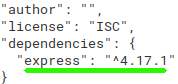
\includegraphics{figuras/dependencies_express.png}
    \caption{Modo como o \gls{NPM} salva no \textit{package.json} a versão de uma dependência}
    \label{fig:dep_express}
\end{figure}{}

Com a informação da versão da dependência no \textit{package.json}, o cliente não precisa se preocupar com as novas atualizações de sua dependência, uma vez que o \gls{NPM}, ao instalar novamente as dependências, sempre irá descarregar a \textit{release} mais recente da dependência que não contenha uma \textit{breaking change}, ou seja, a última \textit{release} disponível para a mesma versão \textit{major} -- desde que a \textit{string} de versionamento seja salva em modo \textit{range}.

\section{Working Tree}
\label{ref-teo:working_tree}

\section{Breaking Change}
\label{ref-teo:breaking_change}